\subsection{Schwarzschild modes \checkmark}
	We now have a look at free fields in the Schwarzschild geometry. For the beginning we need to find a set of modes $f$ that solve the free scalar equation of motion:
		\begin{equation} \label{Klein_Gordon_curved}
			\frac{1}{\sqrt{-g}} \partial_\mu (\sqrt{-g} g^{\mu \nu} \partial_\nu \phi)
			= m^2 \phi
		\end{equation}
	which is the \textit{Klein-Gordons equation for curved space} and where $g_{\mu \nu}$ is the Schwarzschild metric and $g$ is its determinant. Its solutions are also modes in \eqref{wave_fct}, were we can study its properties in an appropriate quantum state such as the Hartle-Hawking state\footnote{The Hartle-Hawking state is the pure state for the Schwarzschild geometry, where the two exteriors of the Rindler space are thermally entangled as seen in the chapter \ref{approxChap} above.}
	
	We now focus on the right exterior of the Schwarzschild geometry, where we use the coordinates $(t,r, \Omega)$. The solutions are having the form
		\begin{equation}
			f_{\omega l m} = 
			\frac{1}{r} Y_{l m}(\Omega) e^{-i \omega t} \psi_{\omega l}(r)
		\end{equation}
	Let's put these into the equation \eqref{Klein_Gordon_curved} above, use the tortoise coordinates from \eqref{r_*tortoise} and plug in
		\begin{align*}
			g^{\mu \nu} &= diag \left(
				\frac{1}{\frac{1}{r}-1},
				1 - \frac{1}{r},
				\frac{1}{r^2},
				\frac{1}{r^2 \sin \theta}
			\right) \\
			\Rightarrow \sqrt{-g}&= r^2 \sin \theta
		\end{align*}
	to reform it into a Schrödinger equation:
		\begin{equation} \label{schroedinger_eq}
			- \frac{d^2}{dr^2_*} \Psi_{\omega l} 
			+ V(r) \Psi_{\omega l} 
			= \omega^2 \Psi_{\omega l}
		\end{equation}
	with the effective Potential of
		\begin{equation}
			V(r)=
			\frac{r-1}{r^3} \left( m^2r^2 + l(l+1) + \frac{1}{r}
			\right)
		\end{equation}
	Let's have a look at the mass m: For simlicity, we consider the Compton wavelength $\frac{1}{m}$ can be\footnote{ The \textit{Schwarzschild radius $r_s$ is still 1}, but I sometimes write $r_s$ to make some things better understandable.} 
		\begin{enumerate}[(i)]
			\item $\frac{1}{m} \ll r_s$	~~ which is the \textit{massive case} and \label{massive}
			\item $\frac{1}{m} \gg r_s$	~~ which is the \textit{massless case}. \label{massless}
		\end{enumerate}
	For to explain, why case \eqref{massless} is more interesting for us, we first need to have a look at case \eqref{massive}.
	
	\begin{figure} [tbp]
			\begin{center}
				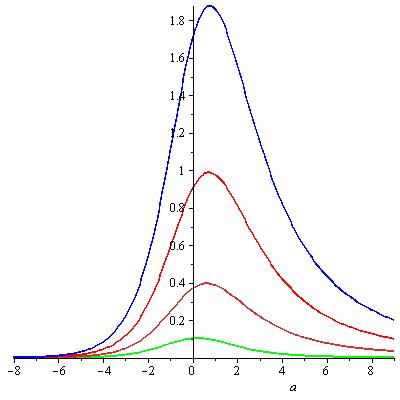
\includegraphics[scale=0.5]{plots_of_V}
				\caption{These are the selfmade plots of $V(r_*)$ for $l=\{0,1,2,3$\}.} \label{plots_of_V}
			\end{center}
	\end{figure} %eigener Plot eingefügen
	Here the potential goes to $m^2$ for $r \gg 1$ which means that massive modes will only propagate till near infinity if $\omega \geq m$. Because we assumed, that $m \gg 1$, any modes with an energy $\omega$ of order of the Schwarzschild radius \textit{will stay near the horizon}. 
	 
	But we found out earlier, that the temperature of black holes is of order $\frac{1}{r_s}$. This means, that $\omega \approx 1$ would be the most interesting energy, but if the mass is already much bigger than one, we cannot examine the propagation to infinity because $\omega$ would also be much bigger than one.
		
	So from now on we remain within the case of $m^2=0$, the massless case.
	Here the asymptotic behavior of the potential is
		\begin{equation} \label{potential_near_infinity}
			V\approx
			\begin{cases}
				\frac{l(l+1)}{r^2_*} &r_* \rightarrow \infty \\
				(l^2 + l + 1) e^{r_*-1} &r_* \rightarrow - \infty
			\end{cases}
		\end{equation}
	If you wonder, why $r_*$ can go to infinity, then send $r$ in the tortoise coordinate \eqref{r_*tortoise} to 1 (which would be the Schwarzschild radius). You will get minus infinity. So this just means, that $r$ approaches $r_s$. 
	
	So the first approachment in \eqref{potential_near_infinity} leads to the vanishment of the potential at spatial infinity polynomially in $r_*$, but near the horizon it vanishes exponentially.
	The barrier between these two regions of \eqref{potential_near_infinity} can be seen in \textbf{Figure \ref{plots_of_V}}. For $\ell \gg 1$ we will find the peak at $r = \frac{3}{2}$ (which means in the figure at approx. $r_*= 0.8$) with a height of order $\ell^2$.
	
	For modes with less energy then the height of the barrier, we have two regions outside the black hole to look at: 
	\begin{enumerate}[1.)]
		\item $r \gg \frac{3}{2}$ : Here the geometry is weakly curved, so modes propagate like in Minkowski space.
		\item $1 < r < \frac{3}{2}$ : This near-horizon region can be called "thermal atmosphere" or "the zone". The first name was given because the modes, which propagate mostly near the horizon, must deal with a Boltzmann distribution with temperature $T_{\text{Hawking}} \approx 1$.  
	\end{enumerate} 	
	If we one approches this problem on the base of Schrödinger equation \eqref{schroedinger_eq}, it can be viewed as a scattering problem, see \textbf{Figure \ref{scattering}}. The modes can come from two directions and leave in two directions namely: coming from a white hole horizon at $r_*\rightarrow -\infty$ or from $J_-$ at $r_*\rightarrow \infty$, which is the past null infinity if you remember, and leaving into the black hole horizon at $r_* \rightarrow -\infty$ or through $J_+$ at $r_* \rightarrow \infty$, which would be the future null infinity.
	
	If we want to know how one unique mode behaves, we need to look set boundary conditions. There are two possible directions, the particles can come from:
	\begin{enumerate}[(i)]
		\item They are send in from the right ({\color{blue} blue} arrow). The possibility if the black hole absorbs them ({\color{red} red} arrow), is given by the transmission coefficient which we get from the Schrödinger problem. But most of them will not ({\color{orange} orange} arrow), so the biggest part of the modes will live at $r \gg 1$.
		\item This time, we don't allow particles come from the right. Instead they are coming out of the white hole, from the left ({\color{forestgreen} green} arrow). Most of it will be reflected off the barrier and fall back into the black hole ({\color{red} red} arrow). Some will tunnel through and go to infinity ({\color{orange} orange} arrow). There the biggest part of these modes is near the horizon which is why they are often called "zone modes" or "modes in the zone".
	\end{enumerate} 
	
	In the following chapter we will find out, which modes are more important.  
	\begin{figure} [tbp]
		\begin{center}
			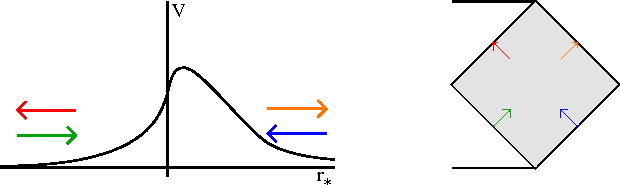
\includegraphics[scale=1.6]{schscat}
			\caption{On the right side there is shown a part of the Schwarzschild Penrose diagram. The grey region is $-\infty < r_* <\infty$. At the left you can see one potential V build on $r_*$ and the possible directions the modes can go are the colorful arrows. The {\color{forestgreen} green} one is coming from the white hole, the {\color{blue} blue} one comes from the null past infinity while the {\color{red} red} one goes into the black hole and the {\color{orange} orange} one goes to the null future infinity.} \label{scattering}
		\end{center}
	\end{figure}